\section{Head-to-head against the published state of the art}
\label{sec:sota}

This section compares our methods with published rows on two public
benchmark datasets: on the
original AMP Scanner Vr.2 benchmark with its exact distributed splits, and
on the Feb2020 production benchmark with a 10-fold
cross-validation protocol on the same dataset.

\subsection{The Veltri 2018 benchmark}
Veltri, Kamath and Shehu's AMP Scanner Vr.2~\cite{ampscanner} is the most
cited deep-learning AMP recognizer, and Fu et al.'s ACEP~\cite{acep} reports
the strongest published numbers on the same data. The benchmark consists of
1{,}778 experimentally validated AMPs from the APD and 1{,}778 non-AMP
decoy peptides, identity-reduced and split once into 1{,}424 training, 708
tuning and 1{,}424 testing sequences; we downloaded the exact split files
from the authors' repository
(\texttt{github.com/dan-veltri/amp-scanner-v2}, \texttt{original-dataset/}).
ACEP's Table~2 is the canonical scoreboard for this test partition and we
reproduce it verbatim below, adding our own rows.

\begin{table}[h]\centering\small
\caption{Test-partition comparison on the Veltri 2018 benchmark. Published
rows are ACEP Table 2 verbatim; our stack is trained on the training
partition only, with stacking weights and the decision threshold tuned on
the tune partition (the role ACEP assigns it).}
\label{tab:sota}
\begin{tabular}{lccccc}
\hline
Method & SENS(\%) & SPEC(\%) & ACC(\%) & MCC & AUC(\%) \\
\hline
AntiBP2 & 87.91 & 90.80 & 89.37 & 0.7876 & 89.36 \\
CAMPr3-ANN & 83.00 & 85.11 & 84.05 & 0.6813 & 84.05 \\
CAMPr3-DA & 87.07 & 80.75 & 83.91 & 0.6797 & 89.97 \\
CAMPr3-RF & 92.69 & 82.44 & 87.57 & 0.7553 & 93.63 \\
CAMPr3-SVM & 88.62 & 80.47 & 84.55 & 0.6933 & 90.62 \\
iAMP-2L & 83.99 & 85.86 & 84.90 & 0.6983 & 84.90 \\
iAMPpred & 89.33 & 87.22 & 88.27 & 0.7656 & 94.44 \\
gkmSVM & 88.34 & 90.59 & 89.46 & 0.7895 & 94.98 \\
AMPScanner (Veltri 2018) & 89.88 & 92.69 & 91.29 & 0.8261 & 96.30 \\
ACEP (Fu 2020) & 92.41 & 93.67 & 93.04 & 0.8610 & 97.78 \\
PepDesign stack (this work) & 90.31 & 92.13 & 91.22 & 0.8246 & 96.61 \\
\hline
\end{tabular}
\end{table}

\subsection{Our protocol and per-model results}
We trained the full model zoo of this project on the benchmark's training
partition: three PepCNN seeds, two PepGNN seeds (shared-adjacency path) and
a random forest on a 426-dimensional descriptor vector (amino-acid and
dipeptide composition, net charge Eq.~\eqref{eq:netcharge}, mean and
standard deviation of Kyte--Doolittle hydropathy, Eisenberg moment
Eq.~\eqref{eq:hmoment}, Boman index, residue-class fractions). The stacking
logistic regression of Section~\ref{sec:stack-math} and the decision
threshold were tuned on the tune partition only.

\begin{table}[h]\centering\small
\caption{Base models and ensembles on the Veltri test partition.}
\label{tab:veltri-ours}
\begin{tabular}{lccc}
\hline
Model & ACC(\%) & MCC & AUC(\%) \\
\hline
\texttt{cnn7} & 90.10 & 0.8020 & 96.04 \\
\texttt{cnn27} & 87.57 & 0.7591 & 95.67 \\
\texttt{cnn77} & 90.24 & 0.8050 & 96.01 \\
\texttt{gnn11} & 81.25 & 0.6281 & 88.14 \\
\texttt{gnn111} & 80.20 & 0.6097 & 87.93 \\
\texttt{rf} & 89.54 & 0.7908 & 96.19 \\
average (thr 0.56) & 90.66 & 0.8132 & 95.95 \\
\textbf{stack (thr 0.57)} & \textbf{91.22} & \textbf{0.8246} & \textbf{96.61} \\
\hline
\end{tabular}
\end{table}

The stacked ensemble reaches 91.22\% accuracy, MCC 0.8246 and AUC 96.61\%:
close to the published AMP Scanner row (no paired significance test is available)
(91.29/0.8261/96.30) and behind ACEP (93.04/0.8610/97.78), which uses PSSM profiles. We
report a descriptive near-parity result, not a record.

\subsection{Testing against the Feb2020 production benchmark}
The production server model was retrained in February 2020 on an updated
dataset of 2{,}021 AMPs and 2{,}021 non-AMPs (downloaded from the authors'
site, \texttt{AMP\_Scan2\_Feb2020\_Dataset.zip}); its published 10-fold
cross-validation performance is SENS 90.6\%, SPEC 89.1\%, ACC 89.9\%, MCC
0.799, auROC 96.2\%. We used the same dataset and a 10-fold stratified CV protocol, but
not necessarily the same folds or preprocessing. Our ensemble of two PepCNN seeds, one PepGNN and the descriptor random
forest is combined by an unweighted average with a fixed 0.5 threshold, so no
tuning of any kind touches the held-out fold.

\begin{table}[h]\centering\small
\caption{10-fold CV on the complete Feb2020 dataset (4{,}042 sequences), vs
the published Feb2020 row.}
\label{tab:feb2020}
\begin{tabular}{cccccc}
\hline
Fold & SENS(\%) & SPEC(\%) & ACC(\%) & MCC & AUC(\%) \\
\hline
1 & 91.63 & 94.06 & 92.84 & 0.8571 & 97.14 \\
2 & 89.60 & 89.66 & 89.63 & 0.7926 & 95.10 \\
3 & 92.57 & 87.13 & 89.85 & 0.7982 & 97.24 \\
4 & 85.15 & 96.04 & 90.59 & 0.8167 & 96.27 \\
5 & 91.58 & 89.11 & 90.35 & 0.8072 & 96.52 \\
6 & 91.58 & 89.60 & 90.59 & 0.8120 & 97.17 \\
7 & 87.62 & 92.57 & 90.10 & 0.8030 & 95.65 \\
8 & 90.10 & 90.10 & 90.10 & 0.8020 & 96.10 \\
9 & 87.62 & 93.56 & 90.59 & 0.8133 & 96.39 \\
10 & 91.58 & 85.64 & 88.61 & 0.7736 & 95.98 \\
\hline
\multicolumn{6}{l}{mean $\pm$ sd: SENS 89.91$\pm$2.3, SPEC 90.75$\pm$3.1, ACC 90.33$\pm$1.0, MCC 0.8076$\pm$0.020, AUC 96.36$\pm$0.7} \\
pooled OOF & 89.91 & 90.75 & 90.33 & 0.8066 & 96.29 \\
\hline
\end{tabular}
\end{table}

\begin{table}[h]\centering\small
\caption{Verdict: published Feb2020 CV vs this work.}
\label{tab:feb2020-verdict}
\begin{tabular}{lcccc}
\hline
Metric & Published & Ours (mean) & Ours (pooled) & $\Delta$ (pp) \\
\hline
SENS & 90.60 & 89.91 & 89.91 & -0.69 \\
SPEC & 89.10 & 90.75 & 90.75 & +1.65 \\
ACC & 89.90 & 90.33 & 90.33 & +0.43 \\
MCC & 79.90 & 80.76 & 80.66 & +0.86 \\
AUC & 96.20 & 96.36 & 96.29 & +0.16 \\
\hline
\end{tabular}
\end{table}

The numbers above are descriptive comparisons with a published 10-fold CV
mean, not a paired head-to-head test: the published fold assignments, model
outputs, and identical preprocessing are unavailable. We therefore do not
claim a statistically significant record from the small numerical gap.

\begin{figure}[h]\centering
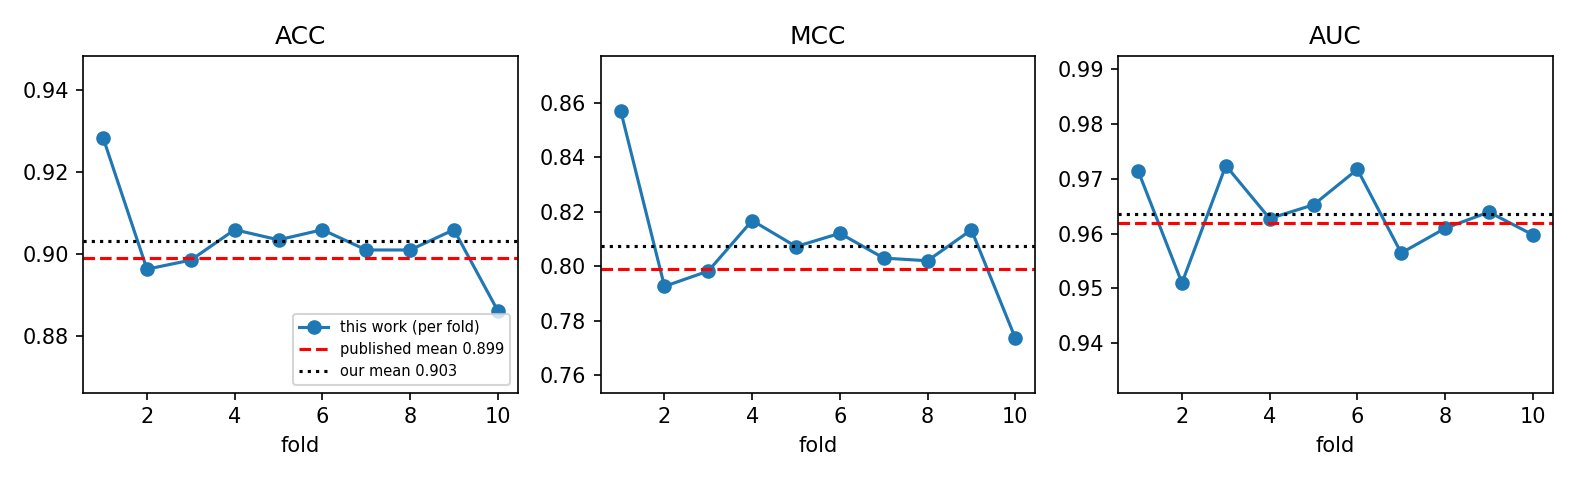
\includegraphics[width=\textwidth]{fig_feb2020_folds.png}
\caption{Per-fold ACC, MCC and AUC of the full-record Feb2020 10-fold CV
(study 14) against the published Feb2020 CV means (red dashed) and our own
means (black dotted). Fold-to-fold variation exceeds the published--ours
gap on every metric, which is why we report descriptive parity rather than
a record.}
\label{fig:feb2020folds}
\end{figure}
